\documentclass[12pt,openright,twoside,a4paper]{book}

\usepackage[T1]{fontenc}
\usepackage[utf8]{inputenc}
\usepackage[brazil]{babel}
\usepackage{lmodern}
\usepackage{microtype}

\usepackage{amsmath,amssymb,mathtools}
\usepackage{siunitx}
\sisetup{
  locale = DE,
  per-mode = symbol,
  separate-uncertainty = true
}

\usepackage{booktabs}
\usepackage{graphicx}
\usepackage{xcolor}
\usepackage{listings}
\usepackage{caption}
\usepackage{subcaption}

\usepackage[
  colorlinks=true,
  linkcolor=blue!50!black,
  citecolor=green!40!black,
  urlcolor=blue!60!black
]{hyperref}
\usepackage[nameinlink,noabbrev,brazilian]{cleveref}

\graphicspath{{figuras/}}

\newcommand{\vetor}[1]{\boldsymbol{#1}}
\newcommand{\dd}{\mathop{}\!\mathrm{d}}
\newcommand{\e}{\mathrm{e}}

\definecolor{corcodigo}{RGB}{30,70,105}
\definecolor{fundocodigo}{RGB}{247,249,251}

\lstdefinestyle{pythonlivro}{
  language=Python,
  basicstyle=\ttfamily\small,
  keywordstyle=\color{corcodigo}\bfseries,
  commentstyle=\color{green!40!black},
  stringstyle=\color{orange!60!black},
  backgroundcolor=\color{fundocodigo},
  frame=single,
  rulecolor=\color{black!20},
  numbers=left,
  numberstyle=\tiny\color{black!55},
  breaklines=true,
  showstringspaces=false,
  columns=fullflexible,
  keepspaces=true
}

\lstset{style=pythonlivro}



% Durante a revisão, descomente para compilar somente um capítulo:
% \includeonly{capitulos/cap01-ferramentas-matematicas}

\begin{document}

\frontmatter
\title{Física com Python}
\author{Sidney Cerqueira}
\date{\the\year}
\maketitle
\tableofcontents

\mainmatter
\chapter{Python: ambiente e fundamentos}
\label{cap:python-fundamentos}

\section{O papel do Python neste livro}

Python é uma linguagem de programação de propósito geral. Neste livro, ela será usada como ferramenta de investigação: realizaremos cálculos, analisaremos dados, construiremos gráficos, desenharemos vetores e simularemos modelos físicos.

O código não substitui a formulação matemática nem a interpretação física. Ele permite executar um procedimento de forma reproduzível e explorar situações que seriam trabalhosas manualmente. Um resultado numérico só se torna fisicamente útil depois que suas unidades, hipóteses e limites são examinados.

Adotaremos o \textbf{Python 3.12}. Versões posteriores da série 3 provavelmente executarão a maior parte dos exemplos, mas a versão 3.12 será nossa referência de desenvolvimento e validação. Fixar uma versão reduz diferenças de comportamento entre computadores e facilita a reprodução dos resultados.

\section{Interpretador, programa e script}

O interpretador Python é o programa que lê e executa instruções escritas na linguagem Python. Uma instrução pode ser digitada em uma sessão interativa ou armazenada em um arquivo de texto com extensão \texttt{.py}.

Um arquivo como

\begin{center}
  \texttt{primeiro\_programa.py}
\end{center}

é chamado de \emph{script}. No terminal integrado do VS Code, ele pode ser executado com

\begin{lstlisting}[language={},numbers=none]
python primeiro_programa.py
\end{lstlisting}

Neste projeto, o interpretador do ambiente virtual pode ser selecionado diretamente pelo VS Code. Isso garante que o editor utilize a mesma versão de Python e as mesmas bibliotecas usadas na validação do livro.

\section{Onde escrever e executar Python}

Python não está vinculado a um único programa. Um arquivo com extensão \texttt{.py} pode ser escrito em diferentes editores e ambientes, desde que um interpretador compatível e as bibliotecas necessárias estejam disponíveis.

É útil distinguir três conceitos:

\begin{itemize}
  \item um \textbf{editor de código} oferece recursos para escrever e organizar arquivos;
  \item uma \textbf{IDE}, ou ambiente integrado de desenvolvimento, reúne editor, execução, depuração, terminal e ferramentas de projeto;
  \item um \textbf{notebook} organiza texto, equações, código e resultados em células executáveis.
\end{itemize}

Entre as alternativas mais conhecidas estão:

\begin{description}
  \item[Visual Studio Code:] editor extensível que, com a extensão Python, oferece execução, depuração, terminal integrado e suporte a notebooks. Será o ambiente principal de validação deste livro.

  \item[JupyterLab:] ambiente local orientado a notebooks. É especialmente útil para exploração de dados, testes rápidos e combinação de explicações com resultados computacionais.

  \item[Google Colab:] serviço executado no navegador e baseado em notebooks. Permite escrever e executar Python sem instalar previamente um ambiente completo no computador. A sessão é remota e temporária; arquivos e bibliotecas instalados durante uma sessão podem não permanecer disponíveis na sessão seguinte.

  \item[PyCharm:] IDE dedicada ao desenvolvimento em Python, com ferramentas de navegação, testes e depuração de projetos.

  \item[Spyder:] IDE voltada à computação científica, com editor, console interativo e visualização de variáveis.
\end{description}

Também é possível executar Python diretamente em um terminal ou utilizar outros editores. A escolha do ambiente não altera as leis físicas nem a sintaxe fundamental da linguagem, mas pode mudar a forma de executar arquivos, instalar bibliotecas e visualizar gráficos.

Os exemplos deste livro serão escritos como scripts Python portáveis. Sempre que um recurso depender especificamente de notebook, VS Code ou Colab, essa dependência será indicada. Para garantir que os resultados publicados possam ser reproduzidos, a validação oficial será realizada no ambiente virtual do projeto com Python 3.12.

\section{O primeiro programa}

A função \texttt{print} envia uma representação de um valor para a saída do programa:

\begin{lstlisting}
print("Fisica com Python")
\end{lstlisting}

O texto entre aspas é uma \emph{string}, isto é, uma sequência de caracteres. Ao executar a instrução, o terminal apresenta

\begin{lstlisting}[language={},numbers=none]
Fisica com Python
\end{lstlisting}

Os parênteses delimitam os argumentos. Aqui, o argumento é uma string.

\section{Valores, variáveis e atribuição}

Uma variável é um nome associado a um valor. A instrução

\begin{lstlisting}
massa = 2.5
\end{lstlisting}

associa o nome \texttt{massa} ao valor numérico \texttt{2.5}. O símbolo \texttt{=} realiza uma \textbf{atribuição}; ele não afirma uma igualdade algébrica permanente.

Depois de

\begin{lstlisting}
velocidade = 3.0
velocidade = 5.0
\end{lstlisting}

o nome \texttt{velocidade} está associado a \texttt{5.0}. A segunda atribuição substitui a referência anterior.

Nomes de variáveis devem comunicar seu significado. Usaremos, por exemplo,

\begin{lstlisting}
tempo_total = 12.0
velocidade_inicial = 4.5
\end{lstlisting}

em vez de nomes genéricos como \texttt{a} ou \texttt{x1}, exceto quando a notação matemática justificar nomes curtos.

O Python não associa unidades físicas automaticamente a números comuns. Por isso, as unidades devem ser declaradas no texto, nos comentários e nos rótulos das saídas:

\begin{lstlisting}
distancia = 120.0  # metros
tempo = 10.0       # segundos
\end{lstlisting}

O caractere \texttt{\#} inicia um comentário. O interpretador ignora o restante daquela linha, mas o comentário ajuda uma pessoa a compreender o programa.

\section{Tipos fundamentais}

Cada valor possui um tipo. Entre os tipos fundamentais estão:

\begin{center}
\begin{tabular}{lll}
\toprule
Tipo & Significado & Exemplo\\
\midrule
\texttt{int} & número inteiro & \texttt{12}\\
\texttt{float} & número de ponto flutuante & \texttt{9.81}\\
\texttt{str} & sequência de caracteres & \texttt{tempo}\\
\texttt{bool} & valor lógico & \texttt{True}, \texttt{False}\\
\bottomrule
\end{tabular}
\end{center}

A função \texttt{type} informa o tipo de um valor:

\begin{lstlisting}
print(type(12))
print(type(9.81))
\end{lstlisting}

A saída esperada é

\begin{lstlisting}[style=saidaesperada]
<class 'int'>
<class 'float'>
\end{lstlisting}

Um \texttt{float} é uma aproximação computacional de um número real. Como sua representação possui precisão finita, algumas operações produzem pequenas diferenças de arredondamento. Esse comportamento será considerado sempre que compararmos resultados numéricos.

\section{Operadores aritméticos}

Os operadores aritméticos básicos são:

\begin{center}
\begin{tabular}{lll}
\toprule
Operador & Operação & Exemplo\\
\midrule
\texttt{+} & adição & \texttt{a + b}\\
\texttt{-} & subtração & \texttt{a - b}\\
\texttt{*} & multiplicação & \texttt{a * b}\\
\texttt{/} & divisão & \texttt{a / b}\\
\texttt{**} & potência & \texttt{a ** 2}\\
\texttt{//} & divisão inteira & \texttt{a // b}\\
\texttt{\%} & resto da divisão & \texttt{a \% b}\\
\bottomrule
\end{tabular}
\end{center}

A precedência das operações é semelhante à utilizada na álgebra. Parênteses devem ser usados quando tornam a intenção mais clara:

\begin{lstlisting}
energia = 0.5 * massa * velocidade**2
media = (medida_1 + medida_2) / 2
\end{lstlisting}

\section{Apresentação de resultados}

Uma \emph{f-string} permite inserir valores em um texto:

\begin{lstlisting}
energia = 9.0
print(f"Energia cinetica: {energia:.2f} J")
\end{lstlisting}

A especificação \texttt{:.2f} apresenta o número com duas casas decimais. A saída será

\begin{lstlisting}[language={},numbers=none]
Energia cinetica: 9.00 J
\end{lstlisting}

Formatar um valor não aumenta a precisão do cálculo. A formatação controla apenas como o número é exibido.

\section{Funções}

Uma função reúne instruções associadas a uma tarefa. Ela pode receber valores de entrada, chamados argumentos, e devolver um resultado:

\begin{lstlisting}
def energia_cinetica(massa, velocidade):
    return 0.5 * massa * velocidade**2
\end{lstlisting}

A palavra \texttt{def} inicia a definição; os dois-pontos abrem um bloco; a indentação identifica as instruções pertencentes à função; e \texttt{return} devolve o resultado.

A função pode ser utilizada por meio de uma chamada:

\begin{lstlisting}
energia = energia_cinetica(2.0, 3.0)
print(energia)
\end{lstlisting}

A saída esperada é

\begin{lstlisting}[style=saidaesperada]
9.0
\end{lstlisting}

Separar um cálculo em uma função reduz repetição, facilita testes e explicita o modelo empregado.

\section{Módulos e bibliotecas}

Um módulo é um arquivo que contém definições Python reutilizáveis. Uma biblioteca é uma coleção organizada de módulos. O comando \texttt{import} torna essas definições disponíveis no programa.

O módulo \texttt{math} pertence à biblioteca padrão, instalada juntamente com o Python:

\begin{lstlisting}
import math

raiz = math.sqrt(25)
angulo = math.radians(30)
\end{lstlisting}

O prefixo \texttt{math.} informa em qual módulo a função foi definida e evita ambiguidades.

Bibliotecas externas são instaladas separadamente. Neste livro, as principais serão:

\begin{itemize}
  \item \textbf{NumPy}: arrays e computação numérica;
  \item \textbf{Matplotlib}: gráficos e visualizações;
  \item \textbf{SciPy}: algoritmos científicos;
  \item \textbf{SymPy}: matemática simbólica.
\end{itemize}

Um exemplo de importação é

\begin{lstlisting}
import numpy as np
import matplotlib.pyplot as plt
\end{lstlisting}

Os nomes \texttt{np} e \texttt{plt} são convenções amplamente utilizadas. Eles são aliases: nomes abreviados associados aos módulos importados.

\section{Arquivos, pastas e caminhos com pathlib}
\label{sec:pathlib}

Os programas que produzem gráficos precisam informar onde os arquivos serão guardados. Um caminho completo preso a uma pasta pessoal faria o código funcionar apenas naquela organização. Para criar caminhos portáteis, usaremos a classe \texttt{Path}, pertencente ao módulo \texttt{pathlib} da biblioteca padrão do Python.

\begin{lstlisting}
from pathlib import Path

pasta_atual = Path.cwd()
print(pasta_atual)
\end{lstlisting}

O método \texttt{Path.cwd()} informa a \textbf{pasta de trabalho atual}: o local a partir do qual o programa está sendo executado. A saída depende do computador e da pasta aberta no terminal. No Windows, ela poderia ser

\begin{lstlisting}[style=saidaesperada]
C:\Users\ana\FisicaComPython\livro
\end{lstlisting}

No Linux ou no Google Colab, o mesmo comando pode produzir algo como

\begin{lstlisting}[style=saidaesperada]
/home/ana/FisicaComPython/livro
\end{lstlisting}

Essas diferenças não exigem alterações no restante do programa. Em vez de escrever manualmente barras próprias de cada sistema, o operador \texttt{/} combina partes de um caminho:

\begin{lstlisting}
pasta_figuras = Path("figuras") / "cap00"
arquivo = pasta_figuras / "meu-grafico.pdf"
\end{lstlisting}

Como o caminho começa com \texttt{figuras} e não com uma unidade de disco ou uma barra inicial, ele é \textbf{relativo}. Se a pasta de trabalho for \texttt{livro}, o arquivo ficará em \texttt{livro/figuras/cap00/meu-grafico.pdf}. O método \texttt{resolve} permite visualizar o caminho completo calculado no computador:

\begin{lstlisting}
print(arquivo.resolve())
\end{lstlisting}

Antes de salvar, precisamos garantir que a pasta exista:

\begin{lstlisting}
pasta_figuras.mkdir(parents=True, exist_ok=True)
\end{lstlisting}

O argumento \texttt{parents=True} autoriza a criação de pastas intermediárias; \texttt{exist\_ok=True} evita um erro quando a pasta já existe. A sequência portátil que adotaremos será, portanto,

\begin{lstlisting}
from pathlib import Path

pasta_figuras = Path("figuras") / "cap00"
pasta_figuras.mkdir(parents=True, exist_ok=True)
arquivo = pasta_figuras / "meu-grafico.pdf"
\end{lstlisting}

Nos códigos oficiais deste livro, o terminal será aberto na pasta \texttt{livro}. Por exemplo,

\begin{lstlisting}[language={},numbers=none]
python codigos/cap00/primeiro_grafico.py
\end{lstlisting}

Assim, os programas guardam os resultados na pasta \texttt{figuras}, dentro de \texttt{livro}.

Se o leitor copiar um script para outro projeto, a mesma instrução criará a pasta \texttt{figuras} no novo local de execução.

Também existe a variável especial \lstinline|__file__|, que informa o arquivo do script. Ela pode ser útil em projetos com estruturas rígidas, mas não está disponível da mesma forma em todos os notebooks. Por isso, os exemplos introdutórios usarão caminhos relativos à pasta de trabalho. No VS Code, no JupyterLab e no Colab, o leitor deve conferir \texttt{Path.cwd()} quando tiver dúvida sobre o destino de um arquivo.

\section{Primeiros gráficos com Matplotlib}
\label{sec:primeiros-graficos}

Um gráfico científico não é apenas uma ilustração: ele representa a relação entre grandezas. Antes de interpretar curvas de posição, velocidade, energia ou campo, precisamos compreender como os dados são convertidos em elementos visuais e como esses elementos são construídos em Python.

Usaremos o módulo \texttt{matplotlib.pyplot}, importado com o alias \texttt{plt}. A biblioteca Matplotlib organiza um gráfico em dois objetos principais:

\begin{description}
  \item[Figura (\texttt{fig}):] a área completa que será exibida ou salva, como uma folha que pode conter um ou mais gráficos;
  \item[Eixos (\texttt{ax}):] a região em que os dados são desenhados, incluindo os eixos coordenados, marcas, rótulos e curvas.
\end{description}

Essa distinção explica a instrução

\begin{lstlisting}
fig, ax = plt.subplots()
\end{lstlisting}

A função \texttt{plt.subplots} cria a figura e um sistema de eixos. Os nomes \texttt{fig} e \texttt{ax} são convenções, não palavras reservadas do Python.

\subsection{Um primeiro gráfico a partir de dados}

Considere posições medidas a cada segundo. Duas listas armazenam os valores correspondentes de tempo e posição. O primeiro elemento de \texttt{tempo} é associado ao primeiro elemento de \texttt{posicao}, e assim sucessivamente.

\lstinputlisting[
  caption={Primeiro gráfico construído a partir de dados de posição e tempo.},
  label={cod:primeiro-grafico}
]{codigos/cap00/primeiro_grafico.py}

A saída textual esperada é

\lstinputlisting[
  style=saidaesperada,
  caption={Saída esperada do primeiro programa gráfico.}
]{codigos/cap00/saidas/primeiro_grafico.txt}

O arquivo produzido pelo programa é mostrado na \cref{fig:primeiro-grafico}.

\begin{figure}[htbp]
  \centering
  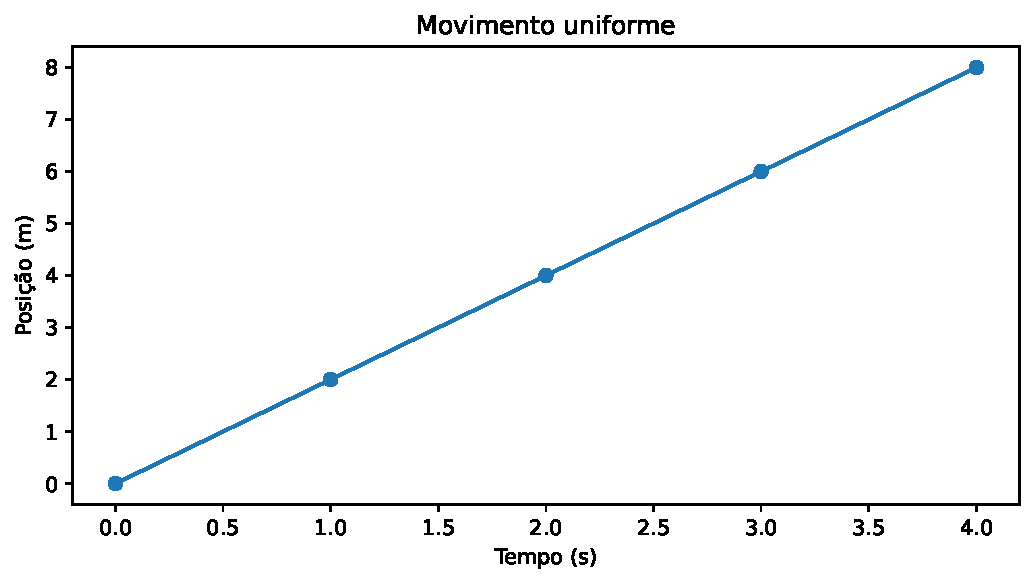
\includegraphics[width=0.78\textwidth]{cap00/primeiro-grafico.pdf}
  \caption{Posição em função do tempo. Os círculos identificam os dados fornecidos ao programa e os segmentos apenas orientam a leitura entre eles.}
  \label{fig:primeiro-grafico}
\end{figure}

No \cref{cod:primeiro-grafico}:

\begin{itemize}
  \item \texttt{ax.plot(tempo, posicao)} associa os valores da primeira sequência ao eixo horizontal e os da segunda ao eixo vertical;
  \item o argumento \texttt{marker="o"} marca cada par de dados com um círculo;
  \item \texttt{set\_xlabel} e \texttt{set\_ylabel} identificam as grandezas e suas unidades;
  \item \texttt{set\_title} acrescenta um título descritivo;
  \item \texttt{tight\_layout} ajusta os espaços para evitar cortes nos rótulos;
  \item \texttt{savefig} salva a figura, enquanto \texttt{plt.close} libera a memória usada por ela.
\end{itemize}

Durante uma exploração interativa, \texttt{plt.show()} pode ser usado para abrir a figura em uma janela ou exibi-la em um notebook. Nos scripts do livro, preferimos \texttt{savefig}: o resultado fica registrado, pode ser reproduzido e pode ser inserido no texto. O formato PDF preserva linhas e letras como elementos vetoriais, adequados à impressão.

\subsection{Amostragem de um intervalo com NumPy}

Listas são suficientes para armazenar uma pequena quantidade de dados experimentais. Para representar uma curva, calculamos a função em muitos pontos.

Por exemplo,

\begin{lstlisting}
tempo = np.linspace(0, 5, 101)
\end{lstlisting}

cria um array NumPy com 101 valores igualmente espaçados, incluindo \num{0} e \num{5}. Um \emph{array} é uma estrutura numérica que permite aplicar uma operação a todos os seus elementos. Assim,

\begin{lstlisting}
posicao = 2.0 * tempo
\end{lstlisting}

calcula uma posição para cada instante sem escrever um laço explicitamente. O conjunto de valores escolhidos para a variável independente é o \textbf{domínio amostrado}. A curva exibida é formada por segmentos entre os pontos calculados; ela não contém infinitos pontos. Aumentar a amostragem pode tornar a curva mais suave, mas não corrige um modelo físico inadequado.

\subsection{Eixos, estilos, legenda, grade e anotação}

Quando duas ou mais curvas aparecem nos mesmos eixos, cada uma precisa ser identificável também em impressão sem cores. Para isso, combinamos rótulos com estilos de linha diferentes.

\lstinputlisting[
  caption={Elementos essenciais de um gráfico científico.},
  label={cod:elementos-grafico}
]{codigos/cap00/elementos_grafico.py}

A saída esperada é

\lstinputlisting[
  style=saidaesperada,
  caption={Saída esperada do programa com duas curvas.}
]{codigos/cap00/saidas/elementos_grafico.txt}

\begin{figure}[htbp]
  \centering
  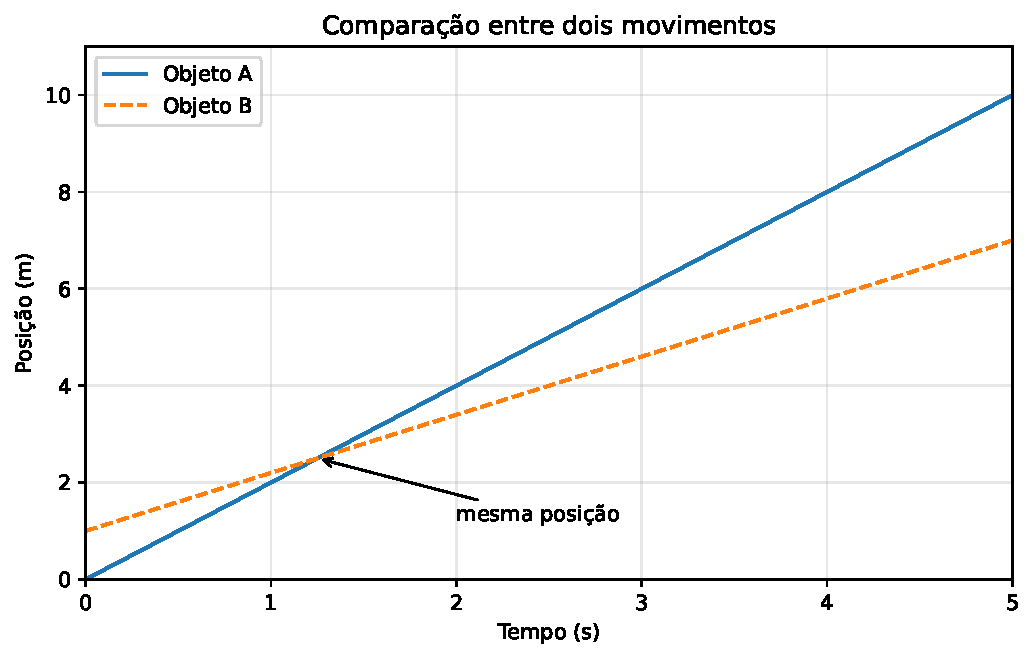
\includegraphics[width=0.82\textwidth]{cap00/elementos-grafico.pdf}
  \caption{Dois movimentos apresentados nos mesmos eixos. Cor, estilo de linha, legenda e anotação trabalham juntos para comunicar a informação.}
  \label{fig:elementos-grafico}
\end{figure}

Os novos comandos controlam diferentes partes da comunicação visual:

\begin{description}
  \item[\texttt{color}:] escolhe a cor da curva;
  \item[\texttt{linestyle}:] define o estilo, como linha contínua ou tracejada;
  \item[\texttt{label}:] associa um texto à curva;
  \item[\texttt{legend}:] exibe os textos associados às curvas;
  \item[\texttt{set\_xlim} e \texttt{set\_ylim}:] definem os limites visíveis dos eixos;
  \item[\texttt{grid}:] acrescenta linhas de referência; o parâmetro \texttt{alpha} controla sua transparência;
  \item[\texttt{annotate}:] relaciona uma observação a um ponto do gráfico. O argumento \texttt{xy} indica o ponto e \texttt{xytext} indica a posição do texto.
\end{description}

Limites de eixos devem ser escolhidos com critério. Cortar parte da escala pode destacar uma variação pequena, mas também pode exagerar visualmente diferenças. Uma grade deve ajudar na leitura, não competir com os dados. Uma legenda é necessária quando há várias curvas sem identificação direta; em uma curva única, bons rótulos de eixos e uma legenda de figura geralmente bastam.

\subsection{Mais de um sistema de eixos}

A função \texttt{plt.subplots} também cria vários gráficos na mesma figura:

\begin{lstlisting}
fig, eixos = plt.subplots(1, 2)
eixos[0].plot(x, y_1)
eixos[1].plot(x, y_2)
\end{lstlisting}

Os argumentos \texttt{1, 2} especificam uma linha e duas colunas. Nesse caso, \texttt{eixos} é uma coleção: \texttt{eixos[0]} seleciona o primeiro sistema de eixos e \texttt{eixos[1]}, o segundo. Esse recurso será usado quando a comparação lado a lado for mais clara do que sobrepor muitas curvas.

\subsection{Linhas de referência, marcas, proporção e formas}

Alguns gráficos exigem mais do que curvas. Os comandos a seguir serão úteis na trigonometria e na representação de vetores:

\begin{lstlisting}
ax.axhline(0)                  # linha horizontal em y = 0
ax.axvline(0)                  # linha vertical em x = 0
ax.set_xticks([0, 1, 2])       # posições das marcas
ax.set_aspect("equal")         # mesma escala visual nos eixos
circulo = plt.Circle((0, 0), 1, fill=False)
ax.add_patch(circulo)          # adiciona a forma aos eixos
ax.quiver(0, 0, 1, 1)         # seta de (0, 0) até (1, 1)
\end{lstlisting}

Os métodos \texttt{axhline} e \texttt{axvline} criam linhas de referência paralelas aos eixos. O método \texttt{set\_xticks} controla onde aparecem as marcas do eixo horizontal; um segundo argumento opcional pode fornecer textos personalizados, como $\pi/2$ e $\pi$. O ajuste \texttt{set\_aspect("equal")} faz uma unidade horizontal ocupar o mesmo comprimento visual que uma unidade vertical, condição necessária para que um círculo não pareça uma elipse.

Uma \texttt{Circle} é uma forma geométrica que só passa a pertencer ao gráfico depois de ser entregue a \texttt{add\_patch}. O método \texttt{quiver} desenha setas e será estudado com mais profundidade quando representarmos vetores. Por enquanto, basta observar que os dois primeiros números indicam a origem e os dois últimos, as componentes da seta.

Textos matemáticos podem ser escritos entre sinais de dólar. Usaremos frequentemente strings como \lstinline|r"$\sin(\theta)$"|. O prefixo \texttt{r} cria uma \emph{raw string}, na qual as barras invertidas são preservadas para a notação matemática do Matplotlib.

\subsection{Critérios para um gráfico científico}

Nem todo cálculo precisa de um gráfico. Ele é útil quando a forma, a tendência, a comparação ou a variação entre grandezas acrescenta informação. Quando for usado, verificaremos se:

\begin{enumerate}
  \item os eixos identificam grandezas e unidades;
  \item o domínio e os limites correspondem ao problema físico;
  \item curvas diferentes podem ser distinguidas sem depender apenas de cor;
  \item a legenda existe somente quando necessária;
  \item a quantidade de pontos representa adequadamente a função ou os dados;
  \item título, grade e anotações ajudam a leitura sem criar excesso visual;
  \item o arquivo foi salvo com resolução ou formato apropriado.
\end{enumerate}

\section{Ambiente virtual e dependências}

Um ambiente virtual isola o interpretador e as bibliotecas de um projeto. Assim, projetos diferentes podem utilizar versões diferentes de uma mesma biblioteca sem interferência entre si.

Neste repositório, o ambiente local fica na pasta \texttt{.venv}. No terminal do VS Code para Windows, ele pode ser ativado com

\begin{lstlisting}[language={},numbers=none]
.\.venv\Scripts\Activate.ps1
\end{lstlisting}

As dependências declaradas no arquivo \texttt{requirements.txt} podem ser instaladas com

\begin{lstlisting}[language={},numbers=none]
python -m pip install -r requirements.txt
\end{lstlisting}

O comando \texttt{python -m pip} garante que o instalador utilizado pertence ao interpretador Python selecionado.

\section{Erros como informação}

Uma mensagem de erro não significa apenas que o programa falhou. Ela registra onde ocorreu o problema e qual regra foi violada. Três categorias aparecerão com frequência:

\begin{itemize}
  \item \texttt{SyntaxError}: a instrução não segue a sintaxe da linguagem;
  \item \texttt{NameError}: um nome foi usado sem estar definido;
  \item \texttt{TypeError}: uma operação recebeu um tipo incompatível.
\end{itemize}

Ao investigar um erro, devemos ler a última linha da mensagem e localizar o arquivo e a linha indicados. Corrigir erros faz parte do processo normal de modelagem computacional.

\section{Critério de validação}

Antes de considerar um código aprovado, verificaremos:

\begin{enumerate}
  \item se o programa executa sem erros;
  \item se as unidades utilizadas são consistentes;
  \item se o resultado coincide com um caso calculado manualmente;
  \item se casos-limite produzem comportamento coerente;
  \item se nomes, comentários e saídas são compreensíveis;
  \item se gráficos possuem eixos, unidades e legendas adequados.
\end{enumerate}

Esses critérios acompanharão todos os códigos do livro.

\chapter{Ferramentas matemáticas para a Física}
\label{cap:ferramentas-matematicas}

\section{Por que começar pela matemática?}

A Física procura descrever regularidades da natureza. Para isso, transforma observações em grandezas mensuráveis e relações entre essas grandezas. A matemática não substitui o fenômeno: ela oferece uma linguagem compacta para formular um modelo, extrair consequências e comparar previsões com medidas.

Considere uma pessoa que caminha em linha reta. A frase ``ela se afasta da origem mantendo o mesmo ritmo'' pode ser representada por

\begin{equation}
  x(t)=x_0+vt,
  \label{eq:posicao-mu}
\end{equation}

em que $x$ é a posição, $t$ é o instante, $x_0$ é a posição inicial e $v$ é a velocidade constante. A equação não é o movimento real; é um modelo que conserva apenas as características relevantes para a pergunta investigada.

Neste capítulo, revisaremos as ferramentas matemáticas que aparecerão repetidamente no livro. O objetivo não é apresentar um curso completo de matemática, mas construir um vocabulário operacional para interpretar equações, gráficos e variações.

\section{Potências e raízes}

Uma potência representa uma multiplicação repetida. Para um expoente inteiro positivo $n$,

\begin{equation}
  a^n=\underbrace{a\cdot a\cdot a\cdots a}_{n\text{ fatores}}.
\end{equation}

Por exemplo,

\begin{equation}
  3^4=3\cdot3\cdot3\cdot3=81.
\end{equation}

Para uma mesma base não nula, valem as propriedades

\begin{align}
  a^m a^n &= a^{m+n},\\
  \frac{a^m}{a^n} &= a^{m-n},\\
  \left(a^m\right)^n &= a^{mn},\\
  a^{-n} &= \frac{1}{a^n},\\
  a^0 &= 1.
\end{align}

Potências fracionárias representam raízes. Para $a\geq0$,

\begin{equation}
  a^{1/2}=\sqrt{a}
\end{equation}

e


\begin{equation}
  a^{1/n}=\sqrt[n]{a}.
\end{equation}

Essas propriedades aparecem frequentemente na manipulação de fórmulas físicas. Se uma grandeza depende de $x^2$, por exemplo, multiplicar $x$ por 3 multiplica essa grandeza por $3^2=9$.

\subsection{Potências em Python}

Em Python, o operador de potência é formado por dois asteriscos, 	exttt{**}. O símbolo 	exttt{\^} não representa potência: ele executa uma operação binária chamada \emph{XOR}.

\lstinputlisting[
  caption={Potências, raízes e uma aplicação à energia cinética.},
  label={lst:potencias-escalas}
]{codigos/cap01/potencias_e_escalas.py}

O valor calculado para $64^{1/3}$ pode aparecer como $3{,}9999999999999996$ em vez de 4. Isso ocorre porque muitos números reais não possuem representação binária finita no computador. A formatação 	exttt{:.2f} controla a apresentação do resultado, mas não altera o valor armazenado.

No trecho final do \cref{lst:potencias-escalas}, triplicamos a velocidade e verificamos numericamente que a energia cinética é multiplicada por nove. O programa, portanto, não apenas calcula um valor: ele testa uma previsão obtida pela análise matemática.

\section{Notação científica e ordem de grandeza}

A Física estuda fenômenos em escalas muito diferentes. O diâmetro aproximado de um próton é da ordem de $10^{-15}\,\si{\meter}$, enquanto a distância entre estrelas pode chegar a muitos trilhões de quilômetros. Escrever números tão pequenos ou tão grandes na forma decimal dificulta cálculos e comparações.

A notação científica representa um número na forma

\begin{equation}
  N=a\times10^n,
  \qquad 1\leq |a|<10,
\end{equation}

em que $n$ é um número inteiro.

Por exemplo,

\begin{equation}
  \SI{0.0000048}{\second}
  =\SI{4.8e-6}{\second}.
\end{equation}

O expoente $-6$ informa que a vírgula foi deslocada seis posições para a direita para obter o número $4{,}8$.

Para um número grande,

\begin{equation}
  \SI{384000000}{\meter}
  =\SI{3.84e8}{\meter}.
\end{equation}

Nesse caso, a vírgula foi deslocada oito posições para a esquerda.

\subsection{Operações com notação científica}

Na multiplicação, multiplicamos os coeficientes e somamos os expoentes:

\begin{equation}
  \left(a\times10^m\right)\left(b\times10^n\right)
  =ab\times10^{m+n}.
\end{equation}

Como exemplo,

\begin{equation}
  \left(3\times10^4\right)\left(2\times10^{-2}\right)
  =6\times10^2.
\end{equation}

Na divisão, dividimos os coeficientes e subtraímos os expoentes:

\begin{equation}
  \frac{a\times10^m}{b\times10^n}
  =\frac{a}{b}\times10^{m-n}.
\end{equation}

Portanto,

\begin{equation}
  \frac{8\times10^7}{2\times10^3}
  =4\times10^4.
\end{equation}

Na adição e na subtração, os expoentes precisam ser iguais. Por exemplo,

\begin{align}
  3{,}2\times10^5+7{,}0\times10^4
  &=3{,}2\times10^5+0{,}7\times10^5\\
  &=3{,}9\times10^5.
\end{align}

\subsection{Ordem de grandeza}

A ordem de grandeza é a potência de dez mais próxima do valor considerado. Ela permite comparar escalas e avaliar rapidamente se um resultado é plausível.

Considere

\begin{equation}
  N=a\times10^n,
  \qquad 1\leq a<10.
\end{equation}

Como o ponto médio entre $10^n$ e $10^{n+1}$, em escala logarítmica, corresponde a $\sqrt{10}\approx3{,}16$, adotamos

\begin{equation}
  \operatorname{OG}(N)=
  \begin{cases}
    10^n, & a<\sqrt{10},\\
    10^{n+1}, & a\geq\sqrt{10}.
  \end{cases}
\end{equation}

Assim, $2{,}4\times10^6$ tem ordem de grandeza $10^6$, enquanto $7{,}1\times10^6$ tem ordem de grandeza $10^7$.

\subsection{Estimativas físicas}

Antes de aceitar o resultado de um cálculo, devemos perguntar:

\begin{itemize}
  \item A unidade está correta?
  \item O sinal possui significado físico?
  \item O valor está na escala esperada?
  \item O resultado respeita os limites do modelo?
\end{itemize}

Uma velocidade cotidiana de $3\times10^7\,\si{\meter\per\second}$ é matematicamente possível como número, mas incompatível com uma caminhada, um automóvel ou um avião. Um resultado assim provavelmente indica erro de unidade, entrada ou interpretação.

\subsection*{Exemplo resolvido}

Um sinal percorre $1{,}5\times10^8\,\si{\meter}$ em $5{,}0\times10^{-1}\,\si{\second}$. Sua velocidade média é

\begin{equation}
  v_m=\frac{\Delta s}{\Delta t}.
\end{equation}

Substituindo,

\begin{align}
  v_m
  &=\frac{1{,}5\times10^8}{5{,}0\times10^{-1}}\\
  &=\frac{1{,}5}{5{,}0}\times10^{8-(-1)}\\
  &=0{,}30\times10^9\\
  &=3{,}0\times10^8\,\si{\meter\per\second}.
\end{align}

Além de efetuar o cálculo, devemos interpretar o resultado. O valor está na ordem de grandeza da velocidade da luz no vácuo, indicando que o modelo pode estar descrevendo a propagação de um sinal eletromagnético.

\subsection*{Verificação conceitual}

\begin{enumerate}
  \item Escreva $0{,}00000032\,\si{\meter}$ em notação científica.
  \item Escreva $6{,}02\times10^{23}$ na forma decimal.
  \item Determine a ordem de grandeza de $2{,}8\times10^5$.
  \item Determine a ordem de grandeza de $8{,}4\times10^5$.
  \item Explique por que a ordem de grandeza é útil para validar resultados físicos.
\end{enumerate}

\section{Proporcionalidade e leis de escala}

As relações de proporcionalidade ajudam a prever como uma grandeza física muda quando outra é alterada. Muitas vezes, essa análise pode ser feita antes de qualquer substituição numérica.

\subsection{Proporcionalidade direta}

Quando escrevemos

\begin{equation}
  y\propto x,
\end{equation}

afirmamos que existe uma constante $k$ tal que

\begin{equation}
  y=kx.
\end{equation}

A razão entre as duas grandezas permanece constante:

\begin{equation}
  \frac{y}{x}=k.
\end{equation}

Se $x$ for multiplicado por um fator $f$, então $y$ será multiplicado pelo mesmo fator:

\begin{equation}
  x'=fx
  \quad\Rightarrow\quad
  y'=fy.
\end{equation}

Por exemplo, se a distância percorrida por um objeto com velocidade constante é

\begin{equation}
  d=vt,
\end{equation}

então, mantendo $v$ constante,

\begin{equation}
  d\propto t.
\end{equation}

Se o intervalo de tempo dobrar, a distância também dobrará.

\subsection{Proporcionalidade com uma potência}

Uma relação mais geral pode ser escrita como

\begin{equation}
  y\propto x^n,
\end{equation}

ou

\begin{equation}
  y=kx^n.
\end{equation}

Quando $x$ é multiplicado por um fator $f$,

\begin{equation}
  x'=fx,
\end{equation}

temos

\begin{equation}
  y'=k(fx)^n=f^nkx^n.
\end{equation}

Portanto,

\begin{equation}
  \frac{y'}{y}=f^n.
\end{equation}

Essa expressão permite prever a mudança de $y$ sem conhecer o valor da constante $k$.

\subsection*{Exemplo resolvido: energia cinética}

A energia cinética de um corpo de massa $m$ e velocidade $v$ é

\begin{equation}
  E_c=\frac{1}{2}mv^2.
\end{equation}

Mantendo a massa constante,

\begin{equation}
  E_c\propto v^2.
\end{equation}

Se a velocidade for triplicada, $v'=3v$. Assim,

\begin{equation}
  \frac{E_c'}{E_c}
  =\left(\frac{v'}{v}\right)^2
  =3^2
  =9.
\end{equation}

Portanto, triplicar a velocidade multiplica a energia cinética por nove. Esse resultado não significa apenas que a energia aumentou. Ele mostra que a dependência quadrática torna o aumento da energia mais rápido que o aumento da velocidade.

\subsection{Proporcionalidade inversa}

Quando

\begin{equation}
  y\propto\frac{1}{x},
\end{equation}

temos

\begin{equation}
  y=\frac{k}{x}.
\end{equation}

Nesse caso, $xy=k$. Se $x$ for duplicado, $y$ será reduzido à metade.

De maneira mais geral,

\begin{equation}
  y\propto\frac{1}{x^n}.
\end{equation}

Se $x$ for multiplicado por $f$, então

\begin{equation}
  \frac{y'}{y}=\frac{1}{f^n}.
\end{equation}

\subsection*{Exemplo resolvido: intensidade e distância}

Considere um modelo idealizado no qual a intensidade $I$ recebida de uma fonte puntiforme é inversamente proporcional ao quadrado da distância $r$:

\begin{equation}
  I\propto\frac{1}{r^2}.
\end{equation}

Queremos comparar a intensidade a uma distância $r$ com a intensidade a uma distância $4r$:

\begin{equation}
  \frac{I(4r)}{I(r)}
  =\frac{1/(4r)^2}{1/r^2}
  =\frac{1}{16}.
\end{equation}

Ao quadruplicar a distância, a intensidade é reduzida a um dezesseis avos do valor inicial. Esse comportamento pode ser compreendido geometricamente: a mesma quantidade emitida pela fonte distribui-se por uma área que cresce proporcionalmente a $r^2$.

\subsection{Proporcionalidade conjunta}

Uma grandeza pode depender de mais de uma variável. Por exemplo,

\begin{equation}
  y\propto\frac{a^2b}{c^3}.
\end{equation}

Nesse caso,

\begin{equation}
  y=k\frac{a^2b}{c^3}.
\end{equation}

Se $a$ dobrar, $b$ for triplicado e $c$ permanecer constante, então

\begin{equation}
  \frac{y'}{y}=2^2\cdot3=12.
\end{equation}

A grandeza $y$ será multiplicada por 12.

\subsection{Isolamento de variáveis}

As fórmulas físicas também precisam ser reorganizadas de acordo com a grandeza procurada. Considere

\begin{equation}
  E_c=\frac{1}{2}mv^2.
\end{equation}

Para isolar $v$, multiplicamos a equação por 2:

\begin{equation}
  2E_c=mv^2.
\end{equation}

Dividimos por $m$:

\begin{equation}
  v^2=\frac{2E_c}{m}.
\end{equation}

Finalmente,

\begin{equation}
  v=\sqrt{\frac{2E_c}{m}}.
\end{equation}

Como $v$ representa o módulo da velocidade, escolhemos a raiz não negativa. Em outros contextos, uma equação quadrática pode admitir soluções positivas e negativas com significados físicos diferentes.

\subsection{Limites de uma proporcionalidade}

Uma proporcionalidade física geralmente vale dentro de determinadas condições. A expressão

\begin{equation}
  F=k\Delta x
\end{equation}

descreve aproximadamente uma mola enquanto ela permanece em seu regime elástico. Um alongamento excessivo pode deformar permanentemente o material, tornando o modelo inadequado.

Portanto, identificar uma proporcionalidade exige também perguntar:

\begin{itemize}
  \item Quais grandezas permanecem constantes?
  \item Em qual intervalo a relação foi observada?
  \item Quais hipóteses foram utilizadas?
  \item Em que situação o modelo deixa de funcionar?
\end{itemize}

\subsection*{Verificação conceitual}

\begin{enumerate}
  \item Se $y\propto x^3$, por qual fator $y$ muda quando $x$ dobra?
  \item Se $y\propto1/x^2$, por qual fator $y$ muda quando $x$ é dividido por 3?
  \item Mantendo a velocidade constante, como a energia cinética varia quando a massa é multiplicada por 5?
  \item Mantendo a massa constante, por qual fator a velocidade deve mudar para que a energia cinética seja multiplicada por 4?
  \item Se $P\propto A^2/(BC)$, determine o fator de mudança de $P$ quando $A$ dobra, $B$ triplica e $C$ é reduzido à metade.
  \item Explique por que uma proporcionalidade matematicamente correta pode deixar de representar um sistema físico real.
\end{enumerate}

\section{Logaritmos e escalas logarítmicas}

O logaritmo responde à seguinte pergunta: a qual expoente devemos elevar uma base para obter determinado número? Se

\begin{equation}
  b^y=x,
\end{equation}

então

\begin{equation}
  y=\log_bx,
\end{equation}

com as condições $b>0$, $b\neq1$ e $x>0$.

Por exemplo, $10^3=1000$ implica

\begin{equation}
  \log_{10}(1000)=3.
\end{equation}

Da mesma forma, $2^{-3}=1/8$ implica

\begin{equation}
  \log_2\left(\frac{1}{8}\right)=-3.
\end{equation}

\subsection{Bases mais utilizadas}

O logaritmo decimal possui base 10:

\begin{equation}
  \log x=\log_{10}x.
\end{equation}

O logaritmo natural possui base $\e\approx2{,}71828$ e é representado por

\begin{equation}
  \ln x=\log_\e x.
\end{equation}

O logaritmo natural aparece naturalmente em processos exponenciais, equações diferenciais, oscilações amortecidas e fenômenos de crescimento ou decaimento.

\subsection{Propriedades fundamentais}

Para $a>0$, $b>0$ e qualquer número real $n$,

\begin{align}
  \log(ab) &= \log a+\log b,\\
  \log\left(\frac{a}{b}\right) &= \log a-\log b,\\
  \log(a^n) &= n\log a.
\end{align}

Também temos $\log_b1=0$ e $\log_bb=1$. Essas propriedades transformam multiplicações em adições, divisões em subtrações e potências em produtos.

\subsection{Mudança de base}

Um logaritmo pode ser convertido de uma base para outra por meio de

\begin{equation}
  \log_bx=\frac{\log_cx}{\log_cb}.
\end{equation}

Em particular,

\begin{equation}
  \log_bx=\frac{\ln x}{\ln b}.
\end{equation}

\subsection{Logaritmos e leis de potência}

Considere uma relação física da forma

\begin{equation}
  y=Cx^n,
\end{equation}

em que $C$ e $n$ são constantes. Aplicando o logaritmo aos dois lados,

\begin{equation}
  \log y=\log C+n\log x.
\end{equation}

Definindo $Y=\log y$ e $X=\log x$, obtemos

\begin{equation}
  Y=nX+\log C.
\end{equation}

Essa é a equação de uma reta. Em um gráfico de $\log y$ em função de $\log x$, a inclinação corresponde ao expoente $n$, e a interseção com o eixo vertical corresponde a $\log C$.

\subsection*{Exemplo resolvido: determinação de uma lei de escala}

Uma grandeza $y$ apresenta os valores

\begin{center}
\begin{tabular}{cc}
\toprule
$x$ & $y$\\
\midrule
2 & 12\\
4 & 48\\
\bottomrule
\end{tabular}
\end{center}

Suponha que $y=Cx^n$. Dividindo as duas equações,

\begin{equation}
  \frac{48}{12}=\frac{C4^n}{C2^n}.
\end{equation}

Logo, $4=2^n$ e, portanto, $n=2$. Usando $x=2$ e $y=12$,

\begin{equation}
  12=C(2)^2,
\end{equation}

de onde $C=3$. Assim, a relação encontrada é

\begin{equation}
  y=3x^2.
\end{equation}

\subsection{Escalas logarítmicas}

Uma escala linear representa diferenças iguais por distâncias iguais. Uma escala logarítmica representa razões iguais por distâncias iguais. Em uma escala logarítmica de base 10, os valores $1$, $10$, $100$ e $1000$ ficam igualmente espaçados porque cada valor é dez vezes maior que o anterior.

Esse tipo de escala é útil quando uma grandeza percorre muitas ordens de magnitude. Ela permite representar valores muito diferentes no mesmo gráfico sem comprimir excessivamente os menores.

\subsection*{Exemplo físico: nível de intensidade sonora}

O nível de intensidade sonora é definido por

\begin{equation}
  \beta=10\log_{10}\left(\frac{I}{I_0}\right),
\end{equation}

em que $\beta$ é medido em decibéis, $I$ é a intensidade sonora e $I_0$ é uma intensidade de referência.

Se $I=1000I_0$, então

\begin{equation}
  \beta=10\log_{10}(1000)=\SI{30}{\decibel}.
\end{equation}

Se a intensidade for multiplicada por 10, o nível aumenta em \SI{10}{\decibel}:

\begin{align}
  \beta'
  &=10\log_{10}\left(\frac{10I}{I_0}\right)\\
  &=10\left[\log_{10}(10)+\log_{10}\left(\frac{I}{I_0}\right)\right]\\
  &=\SI{10}{\decibel}+\beta.
\end{align}

\subsection{Argumentos dimensionais}

O argumento de um logaritmo deve ser adimensional. Por isso, expressões físicas logarítmicas normalmente envolvem razões entre grandezas de mesma dimensão, como

\begin{equation}
  \ln\left(\frac{x}{x_0}\right)
\end{equation}

e

\begin{equation}
  \log_{10}\left(\frac{I}{I_0}\right).
\end{equation}

Uma expressão como $\ln(\SI{3}{\meter})$ não é fisicamente adequada, pois seu argumento ainda possui dimensão de comprimento.

\subsection{Logaritmos e exponenciais como operações inversas}

As funções exponencial e logarítmica desfazem uma à outra:

\begin{equation}
  \ln(\e^x)=x
\end{equation}

e, para $x>0$,

\begin{equation}
  \e^{\ln x}=x.
\end{equation}

\subsection*{Exemplo resolvido: tempo de decaimento}

Considere

\begin{equation}
  N(t)=N_0\e^{-t/\tau}.
\end{equation}

Queremos determinar o instante em que $N(t)=N_0/4$. Substituindo e dividindo por $N_0$,

\begin{equation}
  \frac{1}{4}=\e^{-t/\tau}.
\end{equation}

Aplicando o logaritmo natural,

\begin{equation}
  \ln\left(\frac{1}{4}\right)=-\frac{t}{\tau}.
\end{equation}

Como $\ln(1/4)=-\ln4$, obtemos

\begin{equation}
  t=\tau\ln4\approx1{,}386\tau.
\end{equation}

\subsection*{Verificação conceitual}

\begin{enumerate}
  \item Calcule $\log_{10}(10^{-6})$.
  \item Simplifique $\ln(a^3/b)$.
  \item Resolva $\e^{2x}=7$.
  \item Uma relação experimental obedece a $y=Cx^n$. Quando $x$ dobra, $y$ é multiplicado por oito. Determine $n$.
  \item Por que o argumento de um logaritmo físico deve ser adimensional?
  \item Quantos decibéis são acrescentados quando a intensidade sonora é multiplicada por 100?
  \item Em $N(t)=N_0\e^{-t/\tau}$, determine o instante em que $N=N_0/10$.
\end{enumerate}

\section{Ângulos e trigonometria}

Um ângulo pode ser medido em graus ou radianos. O radiano é a unidade natural do cálculo e relaciona o comprimento de arco $s$ ao raio $r$:

\begin{equation}
  \theta=\frac{s}{r}.
\end{equation}

Uma volta completa corresponde a $2\pi$ radianos ou $360^\circ$. Portanto,

\begin{equation}
  \theta_{\mathrm{rad}}=\theta_{\mathrm{graus}}\frac{\pi}{180}.
\end{equation}

Em um triângulo retângulo,

\begin{equation}
  \sin\theta=\frac{\text{cateto oposto}}{\text{hipotenusa}},\qquad
  \cos\theta=\frac{\text{cateto adjacente}}{\text{hipotenusa}},
\end{equation}

e


\begin{equation}
  \tan\theta=\frac{\sin\theta}{\cos\theta}.
\end{equation}

A identidade fundamental

\begin{equation}
  \sin^2\theta+\cos^2\theta=1
\end{equation}

decorre do teorema de Pitágoras aplicado ao círculo unitário.

\subsection*{Exemplo: componentes de uma força}

Uma força de módulo \SI{80}{\newton} forma um ângulo de $30^\circ$ acima da horizontal. Suas componentes cartesianas são

\begin{align}
  F_x &= F\cos\theta
       = \SI{80}{\newton}\cos 30^\circ
       \approx \SI{69.3}{\newton},\\
  F_y &= F\sin\theta
       = \SI{80}{\newton}\sin 30^\circ
       = \SI{40}{\newton}.
\end{align}

Mais adiante, representaremos essa decomposição com vetores e verificaremos graficamente que $F^2=F_x^2+F_y^2$.

\section{Funções e gráficos}

Uma função associa cada valor permitido da variável independente a um valor da variável dependente. Em Física, a notação $x(t)$ indica que a posição $x$ depende do tempo $t$.

Antes de desenhar um gráfico, devemos identificar:

\begin{enumerate}
  \item as grandezas representadas nos eixos;
  \item as unidades utilizadas;
  \item o domínio fisicamente relevante;
  \item os pontos de interseção com os eixos;
  \item o comportamento crescente, decrescente ou oscilatório;
  \item os limites do modelo.
\end{enumerate}

\subsection{Relação linear}

A função

\begin{equation}
  y=mx+b
\end{equation}

representa uma reta. O coeficiente angular

\begin{equation}
  m=\frac{\Delta y}{\Delta x}
\end{equation}

mede a variação de $y$ por unidade de $x$, enquanto $b$ é o valor de $y$ quando $x=0$.

Na \cref{eq:posicao-mu}, a inclinação de um gráfico $x\times t$ é a velocidade $v$, e a interseção com o eixo vertical é a posição inicial $x_0$. As unidades da inclinação também carregam significado:

\begin{equation}
  [v]=\frac{[x]}{[t]}=\si{\meter\per\second}.
\end{equation}

\subsection{Leis de potência e relações inversas}

Funções como $y=kx^2$ aparecem em movimentos acelerados e energias; funções como $y=k/x^2$ aparecem em modelos de campos produzidos por fontes puntiformes. A forma do gráfico ajuda a distinguir essas relações, mas a interpretação deve respeitar o domínio físico. Uma expressão que diverge em $x=0$ costuma indicar que o modelo idealizado deixou de ser aplicável nessa região.

\subsection{Comportamento exponencial}

Uma função de decaimento possui a forma

\begin{equation}
  y(t)=y_0\e^{-t/\tau},
\end{equation}

onde $\tau$ define a escala temporal. Em $t=\tau$,

\begin{equation}
  y(\tau)=\frac{y_0}{\e}\approx 0{,}368y_0.
\end{equation}

Esse comportamento surge quando a taxa de variação de uma grandeza é proporcional ao próprio valor da grandeza.

\section{Derivada: taxa de variação instantânea}

A taxa média de variação de $f$ entre $x$ e $x+\Delta x$ é

\begin{equation}
  \frac{\Delta f}{\Delta x}
  =\frac{f(x+\Delta x)-f(x)}{\Delta x}.
\end{equation}

Ao considerar intervalos progressivamente menores, definimos a derivada:

\begin{equation}
  \frac{\dd f}{\dd x}
  =\lim_{\Delta x\to 0}
  \frac{f(x+\Delta x)-f(x)}{\Delta x}.
\end{equation}

Geometricamente, a derivada é a inclinação da reta tangente ao gráfico. Fisicamente, seu significado depende das grandezas envolvidas. Para a posição $x(t)$,

\begin{equation}
  v(t)=\frac{\dd x}{\dd t},
\end{equation}

e para a velocidade,

\begin{equation}
  a(t)=\frac{\dd v}{\dd t}
      =\frac{\dd^2x}{\dd t^2}.
\end{equation}

Algumas derivadas frequentes são

\begin{align}
  \frac{\dd}{\dd x}x^n &= nx^{n-1},\\
  \frac{\dd}{\dd x}\sin x &= \cos x,\\
  \frac{\dd}{\dd x}\cos x &= -\sin x,\\
  \frac{\dd}{\dd x}\e^x &= \e^x,\\
  \frac{\dd}{\dd x}\ln x &= \frac{1}{x}.
\end{align}

As fórmulas trigonométricas pressupõem que $x$ esteja em radianos.

\subsection*{Exemplo: movimento não uniforme}

Considere

\begin{equation}
  x(t)=\SI{2}{\meter}
       +\left(\SI{3}{\meter\per\second}\right)t
       +\left(\SI{0.5}{\meter\per\second\squared}\right)t^2.
\end{equation}

Derivando em relação ao tempo,

\begin{equation}
  v(t)=\SI{3}{\meter\per\second}
       +\left(\SI{1}{\meter\per\second\squared}\right)t.
\end{equation}

A aceleração é constante e vale $\SI{1}{\meter\per\second\squared}$. Observe que os coeficientes possuem unidades diferentes para que todos os termos de $x(t)$ tenham dimensão de comprimento.

\section{Integral: acumulação}

A integral definida pode ser entendida como o limite de uma soma de pequenas contribuições. Se conhecemos a velocidade em função do tempo, o deslocamento entre $t_1$ e $t_2$ é

\begin{equation}
  \Delta x=\int_{t_1}^{t_2}v(t)\,\dd t.
\end{equation}

Geometricamente, essa integral corresponde à área algébrica sob o gráfico $v\times t$. Regiões abaixo do eixo temporal contribuem negativamente, o que distingue deslocamento de distância total percorrida.

Algumas integrais elementares são

\begin{align}
  \int x^n\,\dd x &= \frac{x^{n+1}}{n+1}+C,
  \qquad n\neq -1,\\
  \int \frac{1}{x}\,\dd x &= \ln|x|+C,\\
  \int \sin x\,\dd x &= -\cos x+C,\\
  \int \cos x\,\dd x &= \sin x+C,\\
  \int \e^x\,\dd x &= \e^x+C.
\end{align}

A constante $C$ aparece porque funções que diferem apenas por uma constante possuem a mesma derivada.

\subsection*{Exemplo: deslocamento com velocidade variável}

Para $v(t)=\alpha t$, onde $\alpha$ possui unidade de aceleração,

\begin{equation}
  \Delta x
  =\int_0^T \alpha t\,\dd t
  =\frac{1}{2}\alpha T^2.
\end{equation}

O mesmo resultado corresponde à área de um triângulo de base $T$ e altura $\alpha T$ no gráfico de velocidade por tempo.

\section{Máximos, mínimos e interpretação física}

Em um ponto interior onde uma função diferenciável possui máximo ou mínimo local, sua derivada é nula:

\begin{equation}
  f'(x)=0.
\end{equation}

Essa condição identifica pontos candidatos; não basta, sozinha, para classificá-los. Se

\begin{equation}
  f''(x)>0,
\end{equation}

a concavidade é voltada para cima e o ponto é um mínimo local. Se $f''(x)<0$, temos um máximo local. Também é necessário examinar fronteiras do domínio e pontos onde a derivada não existe.

\subsection*{Exemplo: altura máxima}

Uma pequena esfera é lançada verticalmente, e sua altura é descrita pelo modelo

\begin{equation}
  h(t)=\SI{1.2}{\meter}
       +\left(\SI{8}{\meter\per\second}\right)t
       -\frac{1}{2}\left(\SI{9.8}{\meter\per\second\squared}\right)t^2.
\end{equation}

O instante de altura máxima satisfaz $\dd h/\dd t=0$:

\begin{equation}
  8-9{,}8t=0
  \quad\Rightarrow\quad
  t\approx\SI{0.816}{\second}.
\end{equation}

Como $\dd^2h/\dd t^2=-\SI{9.8}{\meter\per\second\squared}$, a concavidade é negativa e o ponto é de máximo. A interpretação física coincide com o cálculo: no ponto mais alto, a velocidade vertical é momentaneamente nula.

\section{Estratégia para resolver problemas}

Uma solução organizada costuma seguir estas etapas:

\begin{enumerate}
  \item identificar a pergunta e o sistema físico;
  \item listar dados, incógnitas e unidades;
  \item desenhar uma representação quando ela ajudar;
  \item declarar hipóteses e escolher um modelo;
  \item desenvolver a solução simbolicamente antes de substituir números;
  \item verificar dimensões, sinal e ordem de grandeza;
  \item interpretar o resultado no contexto do problema;
  \item reconhecer limitações do modelo.
\end{enumerate}

Programas de computador podem automatizar operações e ampliar nossa capacidade de exploração, mas não escolhem sozinhos o sistema, as hipóteses ou o significado físico do resultado. Essa responsabilidade permanece com quem modela.

\section{Síntese}

Neste capítulo:

\begin{itemize}
  \item usamos notação científica e potências para lidar com escalas físicas;
  \item distinguimos proporcionalidade direta, quadrática e inversa;
  \item revisamos logaritmos e trigonometria;
  \item interpretamos gráficos como representações de relações entre grandezas;
  \item associamos derivadas a taxas instantâneas;
  \item associamos integrais a acumulações e áreas algébricas;
  \item usamos derivadas para localizar extremos;
  \item estabelecemos critérios para verificar resultados físicos.
\end{itemize}

\section{Exercícios propostos}

Os exercícios abaixo foram elaborados para este livro.

\begin{enumerate}
  \item Escreva em notação científica o diâmetro de \SI{0.00000032}{\meter}. Em seguida, converta-o para nanômetros.

  \item A energia armazenada em certo sistema é proporcional ao quadrado de uma variável $q$. Por qual fator a energia muda quando $q$ é multiplicada por 3?

  \item A intensidade de um sinal idealizado é inversamente proporcional ao quadrado da distância. Compare a intensidade a \SI{2}{\meter} e a \SI{6}{\meter} da fonte.

  \item Uma força de \SI{120}{\newton} forma $40^\circ$ com o eixo horizontal. Determine suas componentes cartesianas.

  \item Converta $150^\circ$ para radianos e $5\pi/6$ radianos para graus.

  \item Para $x(t)=4+2t-3t^2$, determine as funções velocidade e aceleração. Indique as unidades que os coeficientes devem possuir se $x$ estiver em metros e $t$ em segundos.

  \item A velocidade de um objeto é $v(t)=5-2t$, em unidades do SI. Calcule o deslocamento entre $t=0$ e $t=4\,\si{\second}$. Explique o sinal do resultado usando o gráfico $v\times t$.

  \item Determine os pontos críticos de $f(x)=x^3-6x^2+9x+2$ e classifique-os quando possível.

  \item A temperatura de um corpo é modelada por $T(t)=T_{\mathrm{amb}}+\Delta T_0\e^{-t/\tau}$. Mostre que a taxa de variação de $T-T_{\mathrm{amb}}$ é proporcional ao próprio excesso de temperatura.

  \item Uma reta em um gráfico posição-tempo passa pelos pontos $(\SI{2}{\second},\SI{7}{\meter})$ e $(\SI{8}{\second},\SI{25}{\meter})$. Determine sua inclinação, interprete-a fisicamente e encontre a posição em $t=0$.
\end{enumerate}


% Os próximos capítulos serão incluídos somente após aprovação:
% \include{capitulos/cap02-medidas-e-incertezas}
% \include{capitulos/cap03-vetores}

\backmatter
\chapter{Resoluções das atividades propostas}
\label{cap:solucoes}

\setcounter{equation}{0}
\renewcommand{\theequation}{S.\arabic{equation}}
\newcounter{solucaolistingbase}
\setcounter{solucaolistingbase}{\value{lstlisting}}
\renewcommand{\thelstlisting}{S.\number\numexpr
  \value{lstlisting}-\value{solucaolistingbase}\relax}

As resoluções são organizadas por capítulo e mantêm a numeração dos exercícios no texto principal. Em cada solução, o desenvolvimento matemático precede a substituição numérica. O Python é usado como verificação quando acrescenta valor ao raciocínio.

\section*{Capítulo 1 — Ferramentas matemáticas para a Física}
\addcontentsline{toc}{section}{Capítulo 1 — Ferramentas matemáticas para a Física}

\subsection*{Exercício 1}

Para escrever o diâmetro em notação científica, deslocamos a vírgula sete posições para a direita:

\begin{equation}
  \SI{0.00000032}{\meter}
  =\SI{3.2e-7}{\meter}.
\end{equation}

Como \(\SI{1}{\meter}=\SI{1e9}{\nano\meter}\), multiplicamos o valor em metros por \(10^9\):

\begin{equation}
  (3{,}2\times10^{-7}\,\si{\meter})
  \left(10^9\,\frac{\si{\nano\meter}}{\si{\meter}}\right)
  =3{,}2\times10^2\,\si{\nano\meter}
  =\SI{320}{\nano\meter}.
\end{equation}

Portanto, o diâmetro é \(\boxed{\SI{3.2e-7}{\meter}=\SI{320}{\nano\meter}}\).

\subsection*{Exercício 2}

Se a energia \(E\) é proporcional a \(q^2\), podemos escrever \(E=Cq^2\), onde \(C\) permanece constante. Ao substituir \(q\) por \(3q\), obtemos

\begin{equation}
  E'=C(3q)^2=9Cq^2=9E.
\end{equation}

Logo, a energia é \(\boxed{9}\) vezes maior.

\subsection*{Exercício 3}

Para uma intensidade \(I\) inversamente proporcional a \(r^2\), temos \(I=C/r^2\). Assim,

\begin{equation}
  \frac{I(\SI{2}{\meter})}{I(\SI{6}{\meter})}
  =\frac{C/2^2}{C/6^2}
  =\frac{6^2}{2^2}
  =9.
\end{equation}

A intensidade a \(\SI{2}{\meter}\) é, portanto, \(\boxed{9}\) vezes a intensidade a \(\SI{6}{\meter}\). Equivalentemente, \(I(\SI{6}{\meter})=I(\SI{2}{\meter})/9\).

\subsection*{Exercício 4}

Tomando o ângulo a partir do eixo horizontal,

\begin{align}
  F_x &= F\cos\theta
       =\SI{120}{\newton}\cos 40^\circ
       \approx\SI{91.9}{\newton},\\
  F_y &= F\sin\theta
       =\SI{120}{\newton}\sin 40^\circ
       \approx\SI{77.1}{\newton}.
\end{align}

As duas componentes são positivas porque o vetor está no primeiro quadrante. Portanto,

\begin{equation}
  \boxed{\vetor{F}\approx
  (\SI{91.9}{\newton})\,\hat{\vetor{\imath}}
  +(\SI{77.1}{\newton})\,\hat{\vetor{\jmath}}}.
\end{equation}

Como verificação, \(\sqrt{F_x^2+F_y^2}\approx\SI{120}{\newton}\).

\subsection*{Exercício 5}

Para converter graus em radianos, multiplicamos por \(\pi/180^\circ\):

\begin{equation}
  150^\circ\frac{\pi\,\si{\radian}}{180^\circ}
  =\boxed{\frac{5\pi}{6}\,\si{\radian}}.
\end{equation}

No sentido inverso,

\begin{equation}
  \frac{5\pi}{6}\,\si{\radian}
  \frac{180^\circ}{\pi\,\si{\radian}}
  =\boxed{150^\circ}.
\end{equation}

Os resultados são consistentes porque as duas expressões representam o mesmo ângulo.

\subsection*{Exercício 6}

A velocidade é a derivada da posição em relação ao tempo:

\begin{equation}
  v(t)=\frac{\dd x}{\dd t}=2-6t.
\end{equation}

A aceleração é a derivada da velocidade:

\begin{equation}
  a(t)=\frac{\dd v}{\dd t}=-6.
\end{equation}

Se \(x\) é medido em metros e \(t\) em segundos, cada termo de \(x(t)\) precisa ter unidade de comprimento. Portanto, o termo constante \(4\) tem unidade de metro, o coeficiente \(2\) tem unidade de \(\si{\meter\per\second}\), e o coeficiente \(-3\) tem unidade de \(\si{\meter\per\second\squared}\). Assim,

\begin{align}
  v(t)&=\boxed{(2-6t)\,\si{\meter\per\second}},\\
  a(t)&=\boxed{-6\,\si{\meter\per\second\squared}}.
\end{align}

Na primeira expressão, os números carregam as unidades necessárias para que ambos os termos representem velocidade.

\subsection*{Exercício 7}

O deslocamento é a integral da velocidade:

\begin{align}
  \Delta x
  &=\int_0^4(5-2t)\,\dd t\\
  &=\left[5t-t^2\right]_0^4\\
  &=20-16\\
  &=\boxed{\SI{4}{\meter}}.
\end{align}

No gráfico \(v\times t\), a velocidade se anula em \(t=\SI{2.5}{\second}\). Entre \(0\) e \(\SI{2.5}{\second}\), a área triangular positiva vale

\begin{equation}
  A_+=\frac{1}{2}(\SI{2.5}{\second})(\SI{5}{\meter\per\second})
  =\SI{6.25}{\meter}.
\end{equation}

Entre \(\SI{2.5}{\second}\) e \(\SI{4}{\second}\), a região fica abaixo do eixo e contribui com

\begin{equation}
  A_-=-\frac{1}{2}(\SI{1.5}{\second})(\SI{3}{\meter\per\second})
  =-\SI{2.25}{\meter}.
\end{equation}

Logo, \(\Delta x=A_++A_-=\SI{4}{\meter}\). O sinal positivo indica que, apesar da inversão do movimento após \(\SI{2.5}{\second}\), o deslocamento no sentido positivo foi maior.

\subsection*{Exercício 8}

Os pontos críticos de uma função diferenciável ocorrem onde \(f'(x)=0\). Para

\begin{equation}
  f(x)=x^3-6x^2+9x+2,
\end{equation}

temos

\begin{equation}
  f'(x)=3x^2-12x+9=3(x-1)(x-3).
\end{equation}

Portanto, os valores críticos são \(x=1\) e \(x=3\). A segunda derivada é

\begin{equation}
  f''(x)=6x-12.
\end{equation}

Em \(x=1\), \(f''(1)=-6<0\), logo há um máximo local. Como \(f(1)=6\), o ponto é \(\boxed{(1,6)}\).

Em \(x=3\), \(f''(3)=6>0\), logo há um mínimo local. Como \(f(3)=2\), o ponto é \(\boxed{(3,2)}\).

\subsection*{Exercício 9}

Definimos o excesso de temperatura em relação ao ambiente como

\begin{equation}
  \Theta(t)=T(t)-T_{\mathrm{amb}}
  =\Delta T_0\e^{-t/\tau}.
\end{equation}

Derivando em relação ao tempo,

\begin{align}
  \frac{\dd\Theta}{\dd t}
  &=-\frac{\Delta T_0}{\tau}\e^{-t/\tau}\\
  &=-\frac{1}{\tau}\Theta.
\end{align}

Como \(\Theta=T-T_{\mathrm{amb}}\), concluímos que

\begin{equation}
  \boxed{\frac{\dd}{\dd t}(T-T_{\mathrm{amb}})
  =-\frac{1}{\tau}(T-T_{\mathrm{amb}})}.
\end{equation}

A taxa é proporcional ao próprio excesso de temperatura. O sinal negativo indica que, para um corpo inicialmente mais quente que o ambiente, o excesso diminui com o tempo.

\subsection*{Exercício 10}

A inclinação da reta posição-tempo é

\begin{equation}
  v=\frac{\Delta x}{\Delta t}
  =\frac{\SI{25}{\meter}-\SI{7}{\meter}}
         {\SI{8}{\second}-\SI{2}{\second}}
  =\boxed{\SI{3}{\meter\per\second}}.
\end{equation}

Essa inclinação representa a velocidade constante. Escrevendo a posição como \(x(t)=x_0+vt\) e usando o ponto \((\SI{2}{\second},\SI{7}{\meter})\), obtemos

\begin{equation}
  \SI{7}{\meter}=x_0+
  (\SI{3}{\meter\per\second})(\SI{2}{\second}),
\end{equation}

de onde

\begin{equation}
  \boxed{x_0=\SI{1}{\meter}}.
\end{equation}

Portanto, a equação da posição é \(\boxed{x(t)=1+3t}\), com \(x\) em metros e \(t\) em segundos.

\subsection*{Verificação numérica em Python}

O programa a seguir confere os resultados numéricos dos exercícios 1, 4, 5, 7, 8 e 10. Ele não substitui os desenvolvimentos anteriores: apenas executa as operações depois que o modelo já foi estabelecido.

\lstinputlisting[
  caption={Verificação numérica de resultados selecionados do Capítulo 1.},
  label={cod:verificacao-solucoes-cap01}
]{codigos/solucoes/verificacao_cap01.py}

A saída esperada é

\lstinputlisting[
  style=saidaesperada,
  caption={Saída esperada da verificação das soluções do Capítulo 1.}
]{codigos/solucoes/saidas/verificacao_cap01.txt}


\end{document}
